% %============
%%  ** Author: Shepherd Qirong
%%  ** Date: 2021-12-04 21:11:37
%%  ** Github: https://github.com/ShepherdQR
%%  ** LastEditors: Shepherd Qirong
%%  ** LastEditTime: 2021-12-04 21:32:36
%%  ** Copyright (c) 2019--20xx Shepherd Qirong. All rights reserved.
%%============


\documentclass[UTF8]{article}
\usepackage{ctex}
\usepackage{amsmath,amsthm,amsfonts,amssymb,bm,mathrsfs,upgreek} 
\usepackage{graphicx}
\usepackage[paper=a4paper,top=3.5cm,bottom=2.5cm,
left=2.7cm,right=2.7cm,
headheight=1.0cm,footskip=0.7cm]{geometry}
\usepackage{color}
\usepackage{multirow,booktabs}

\RequirePackage{setspace}%%linespace
\setstretch{1.523}


\begin{document}
\section{Introduction}
Today is 20211204, and I deciede to note down all of my knowledge about the math in this notebook.

\section{Space}

\subsection{Operation Defination}

\subsubsection{Element}

we define the basic element $\boldsymbol x = [x_1, x_2,\dots]^T = \Sigma x_i \boldsymbol{e_i}$, $ \boldsymbol e_i $ means $x_i = 1, x_j = 0$ for all $j \neq i$. We define Kronecker sign to simply the description of $\boldsymbol e_i \cdot \boldsymbol e_j $.

\begin{equation}
    \begin{split}
    &\delta _{i,j}:=
    \begin{cases}
    &1,\qquad i = j\\
    &0,\qquad i \neq j\\
    \end{cases}\\
    \end{split}
\end{equation}

The set of bases $\{ \boldsymbol e_i  \}  \stackrel{apply}{\longrightarrow} \boldsymbol{x} \longrightarrow    \{ x_i \}    $.




\subsubsection{Dot Product}

We define in algebra, $ \boldsymbol{x} \cdot \boldsymbol{y} := \sum{x_iy_i\boldsymbol{e}_i} = \boldsymbol{x}^T \cdot \boldsymbol{y}$.

Then the defination is restricted to the choose of the coordinate system. We take a look a the product with reflect $T : \boldsymbol x \rightarrow  \boldsymbol{T} \cdot \boldsymbol{x}$,

\begin{equation}
    (\boldsymbol A \cdot \boldsymbol  B)^T = (a_{ik}b_{kj})^T = c_{ij}^T = c_{ji} = b_{jk}a_{ki} = \boldsymbol B^T \cdot \boldsymbol A^T
\end{equation}
we have 
\begin{equation}
    (\boldsymbol T \cdot \boldsymbol  x)^T(\boldsymbol T \cdot \boldsymbol  y) =  \boldsymbol x^T (\boldsymbol T^T \boldsymbol T) \boldsymbol y = [(\boldsymbol T^T \boldsymbol T) \boldsymbol x]^T \boldsymbol y
\end{equation}

We name T a Contractive mapping when $\boldsymbol T^T \boldsymbol T \leqslant   \theta, 0 \leqslant \theta \leqslant 1$.

\subsubsection{geometry Properties}

\begin{equation}
    \begin{split}
    &\parallel \boldsymbol{x} \parallel := \sqrt{\boldsymbol x \cdot \boldsymbol x}\\
    &\cos {\theta_{x,y}} : = \frac
    {\boldsymbol x \cdot \boldsymbol x}
    {\parallel \boldsymbol{x} \parallel \cdot \parallel \boldsymbol{y} \parallel}\\
\end{split}
\end{equation}

\subsubsection{Add}

\begin{equation}
    \begin{split}
    & \boldsymbol x + \boldsymbol y := \sum (x_i + y_i)\boldsymbol e_i\\
    & k \cdot \boldsymbol x := \sum kx_i\boldsymbol e_i\\
\end{split}
\end{equation}

Law $\boldsymbol{x} + \boldsymbol{y} = \boldsymbol{y} + \boldsymbol{x}$,
law $ (\boldsymbol{x} + \boldsymbol{y} )+ \boldsymbol{z} = \boldsymbol{x} +( \boldsymbol{y} + \boldsymbol{z})$ is not obvious in the view of Set Theory.





\begin{figure*}[h]
    \centering
    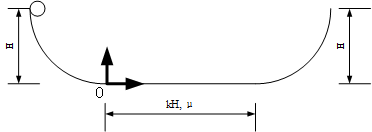
\includegraphics[width=0.5\textwidth]{../../resources/T0001.png}
    \caption{正则项的几何意义}
    \label{fig:1}
\end{figure*}




\end{document}